\documentclass[a4paper,10pt]{article}
\usepackage[utf8]{inputenc}
\usepackage[english] {babel}
\usepackage[T1]{fontenc}
\usepackage{lmodern}
\usepackage{graphicx}
\usepackage{graphics}
\usepackage{ulem}
\usepackage{amssymb}
\usepackage{url}
\usepackage[a4paper]{geometry}
\geometry{hscale=0.7,vscale=0.7,centering}
\usepackage{vmargin}
\usepackage{amsmath}
\usepackage{amssymb}
\usepackage{amsthm}
\usepackage{moreverb}
\usepackage{listings}
\usepackage{enumerate}
%\usepackage{enumitem}
\newtheorem{theorem}{Théorème}[section]
\newtheorem{defi}{Définition}[section] 
\newtheorem{prop}{Propriété}[section] 
\usepackage{color}
\definecolor{gris}{rgb}{0.95,0.95,0.95}
\lstset{numbers=left, tabsize=4, backgroundcolor=\color{gris},
frame=single, breaklines=true,
keywordstyle=\color{black},
stringstyle=\ttfamily,
framexleftmargin=6mm, xleftmargin=6mm}
%opening
\title{LINGI 2261 : Artificial Intelligence \\
Assignement 3 - Mid-Project}
\author{Rochet Florentin - Debroux Léonard} 
\date{Année académique 2011-2012}

\begin{document}

	\begin{titlepage}
		\begin{center}
			{\huge LINGI2261: Artificial Intelligence}\\
			\vspace{0.4cm}
			
			{\Large {Professor : Yves Deville\\ \vspace{0.2cm} Teaching assistants : Cyrille Dejemeppe and Jean-Baptiste Mairy  }}\\
			\vspace{0.6cm}
			
			{\Large \textit{Assignment 4 : Local Search and Propositional Logic}}\\
			\vspace{1.2cm}

			\texttt{}\\
			\vspace{0.2cm}

			
\includegraphics[height=10cm]{pageGarde.png}\\
			\vspace{0.1cm}
			{\Large \textbf{Universit\'e Catholique de Louvain}}
			\vspace{0.7cm}

			Groupe 37 \\
			\vspace{0.2cm}
			
			Florentin Rochet \\
			Léonard Debroux\\
			\vspace{0.2cm}
			2012-2013\\
		\end{center}
	\end{titlepage}

	\newpage
	
\section{The Traveling Salesman Problem}
\subsection{Diversification versus Intensification}
\subsubsection{Question 1}
The point is to find a solution that is as good as possible, while avoiding the bad complexity of the exact solution of the TSP. 
We'll formulate each state as a list of ordered cities and a variable containing the sum of the cost of the distances between two adjacent cities in the list.\\
A solution will be a tuple containing the list of cities, which order follows the indexes in the list, and a double containing the total cost of the solution).\\
The successor function will take an admissible path for the tsp and yield all the possible swaps of two cities in the list.\\
Symmetrical states will be avoided by considering that the swaps of two cities $(c1, c2)$ and $(c2, c1)$ are the same.\\
As said before, the evaluation function sums the distance between each couple of $p_{i}, p_{i+1}$ in the list to give the total cost of the solution.
The distances are recovered from the distance matrix given in the input file.
\subsubsection{Question 2}
The implementation of the tree different strategies are in the python modules: \verb@randomwalk.py@, \verb@maxvalue.py@ and \verb@randomized_maxvalue.py@.
\subsubsection{Question 3}
%\begin{itemize}[noitemsep,nolistsep]
\begin{itemize}
\itemsep0em
\item Algo1 stands for randomwalk.py
\item Algo2 stands for maxvalue.py
\item Algo3 stands for randomzied\_maxvalue.py \\
\end{itemize}
\begin{center}
\begin{tabular}{|c|c|c|c|}
\hline 
att48.tsp & Algo1 & Algo2 & Algo3 \\ 
\hline 
Comp time [s] & 0.57 & 3.39 & 3.468 \\ 
\hline 
Best sol. & 130045.8 & 45336.2 & 42241.96 \\ 
\hline 
\# Steps & 21.6 & 37 & 92.6 \\ 
\hline 
\end{tabular} 
\end{center}
\begin{center}
\begin{tabular}{|c|c|c|c|}
\hline 
bayg29.tsp & Algo1 & Algo2 & Algo3 \\ 
\hline 
Comp time [s] & 0.192 & 0.82 & 0.852 \\ 
\hline 
Best sol. & 21735.1 & 9487.1 & 10413.2 \\ 
\hline 
\# Steps & 34.8 & 21 & 63.2 \\ 
\hline 
\end{tabular} 
\end{center}
\begin{center}
\begin{tabular}{|c|c|c|c|}
\hline 
bays29.tsp & Algo1 & Algo2 & Algo3 \\ 
\hline 
Comp time [s] & 0.186 & 0.8 & 0.857 \\ 
\hline 
Best sol. & 21477.46 & 9487.1 & 10165.5 \\ 
\hline 
\# Steps & 58.8 & 21 & 92.4 \\ 
\hline 
\end{tabular} 
\end{center}
\begin{center}
\begin{tabular}{|c|c|c|c|}
\hline 
berlin52.tsp & Algo1 & Algo2 & Algo3 \\ 
\hline 
Comp time [s] & 0.703 & 4.17 & 4.29 \\ 
\hline 
Best sol. & 24105.5 & 9920.1 & 9240.22 \\ 
\hline 
\# Steps & 7.8 & 42 & 86.8 \\ 
\hline 
\end{tabular} 
\end{center}
\begin{center}
\begin{tabular}{|c|c|c|c|}
\hline 
dantzig42.tsp & Algo1 & Algo2 & Algo3 \\ 
\hline 
Comp time [s] & 0.424 & 2.27 & 2.33 \\ 
\hline 
Best sol. & 946 & 720.8 & 707.5 \\ 
\hline 
\# Steps & 0.0 & 14 & 68.8 \\ 
\hline 
\end{tabular} 
\end{center}

\subsubsection{Question 4}
\begin{center}
\begin{figure}[ht]
		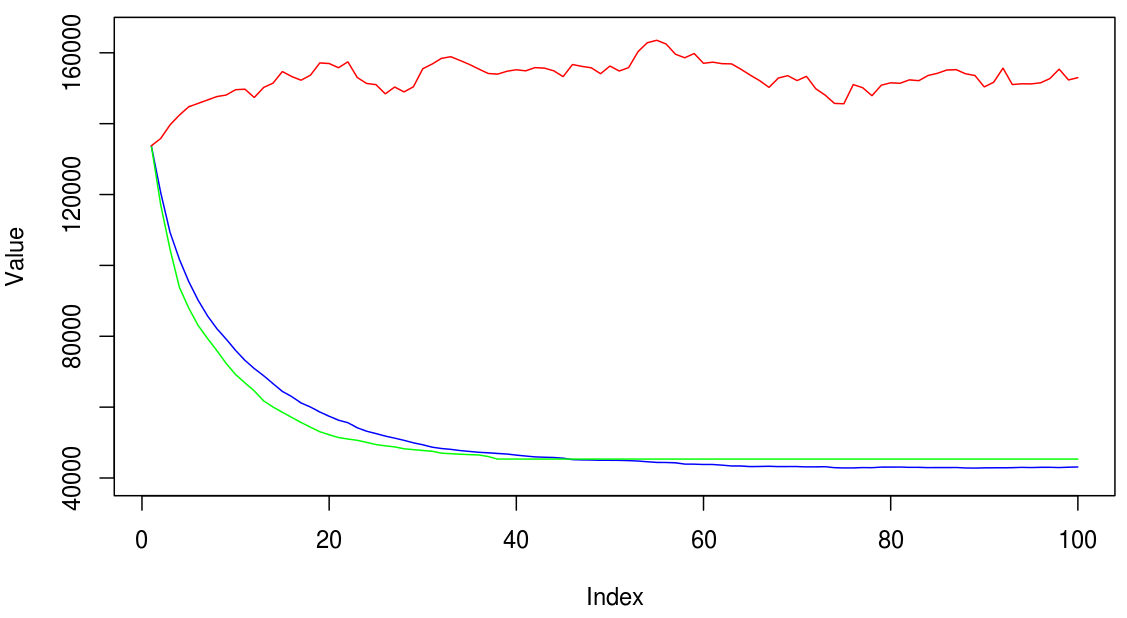
\includegraphics[scale=.35]{mile4_1_1.png}
	\caption{Value by step.py}
\end{figure}
\end{center}
When randomness was part of the algorithms, there were 5 tests for each one (like we did for the third question). The red curve is the \texttt{randomwalk}, the green one is \texttt{maxvalue} and the blue one is \texttt{randomized\_maxvalue}.

\subsubsection{Question 5}
	\begin{enumerate}[(a)]
		\item \texttt{randomized\_maxvalue both} wins by a few over \texttt{maxvalue} and \texttt{randomwalk} is realy bad.
		\item \texttt{randomize\_maxvalue} wins because it mixes randomness and going for the best path, so it will avoid local optima.
		\item The limitation of \texttt{randomwalk} is that it does not look for a good path, so there is less chance to find the best one.\\
		Concerning \texttt{maxvalue}, it falls into a local optimum and is stuck in it.
		\texttt{randomized\_maxvalue} should be the best as it can easily avoid local optima and so, have a chance to find the global one.
		\item It continues to look for a step only to improve the current solution, but as none exists, the current states stays the same for the remaining steps.
		\item There must be a trade off between intensification and diversification because intensification ensures that we go for a good solution, while diversification ensures that we explore several possibilities. \\
		Intensification alone (\verb@maxvalue.py@) would cause the solution to find a local optimum without considering others paths to better solutions and diversification alone (\verb@randomwalk.py@) would cause to explore other paths but no necessarily the good ones.
	\end{enumerate}

\subsection{Some well-known strategies}
\subsubsection{Question 1}
\subsubsection{Question 2}
\subsubsection{Question 3}

\begin{center}
\begin{tabular}{|c|c|c|c|c|c|}
\hline 
att48.tsp & Tabu3 & Tabu3 & Tabu3 & Tabu3 & Sim\_ann \\ 
\hline 
Comp time [s] & 3.52 & 3.52 & 3.51 & 3.5 & 0.59 \\ 
\hline 
Best sol. & 42603.84 & 40772.16 & 42079.8 & 42278.1 & 93831.16 \\ 
\hline 
\# Steps & 91.8 & 89.4 & 96.2 & 88.8 & 97.2 \\ 
\hline 
\end{tabular} 
\end{center}

\begin{center}
\begin{tabular}{|c|c|c|c|c|c|}
\hline 
bayg29.tsp & Tabu3 & Tabu3 & Tabu3 & Tabu3 & Sim\_ann\\ 
\hline 
Comp time [s] & 0.88 & 0.89 & 0.886 & 0.89 & 0.19 \\ 
\hline 
Best sol. & 10020.96 & 9773.64 & 9930.78 & 10082.56 & 16493.74 \\ 
\hline 
\# Steps & 77.2 & 80.2 & 84.8 & 91 & 89.6 \\ 
\hline 
\end{tabular} 
\end{center}

\begin{center}
\begin{tabular}{|c|c|c|c|c|c|}
\hline 
bays29.tsp & Tabu3 & Tabu3 & Tabu3 & Tabu3 & Sim\_ann\\ 
\hline 
Comp time [s] & 0.89 & 0.88 & 0.88 & 0.88 & 0.19 \\ 
\hline 
Best sol. & 10399.12 & 9938.8 & 10067.76 & 10410.68 & 15445.54 \\ 
\hline 
\# Steps & 71.6 & 72 & 94.6 & 83.4 & 88.2 \\ 
\hline 
\end{tabular} 
\end{center}

\begin{center}
\begin{tabular}{|c|c|c|c|c|c|}
\hline 
berlin52.tsp & Tabu3 & Tabu3 & Tabu3 & Tabu3 & Sim\_ann\\ 
\hline 
Comp time [s] & 4.45 & 4.39 & 4.45 & 4.43 & 0.7 \\ 
\hline 
Best sol. & 9737.52 & 9681.32 & 9709.02 & 9481.64 & 19083.78 \\ 
\hline 
\# Steps & 91.6 & 84 & 89.8 & 91.8 & 96.4\\ 
\hline 
\end{tabular} 
\end{center}

\begin{center}
\begin{tabular}{|c|c|c|c|c|c|}
\hline 
dantzig42.tsp & Tabu3 & Tabu3 & Tabu3 & Tabu3 & Sim\_ann\\ 
\hline 
Comp time [s] & 2.42 & 2.47 & 2.42 & 2.46 & 0.42 \\ 
\hline 
Best sol. & 706.02 & 715.5 & 713.58 & 716.36 & 929 \\ 
\hline 
\# Steps & 76 & 75.6 & 60.2 & 56.4 & 45.4 \\ 
\hline 
\end{tabular} 
\end{center}
\texttt{tabu} presents similar results to the previous methods while simulated annealing does not perform so well. We ran for each instance and each algorithm 5 times to have a mean in order to better represent the performance of the algorithms.
\subsubsection{Question 4}
\begin{center}
\begin{figure}[ht]
		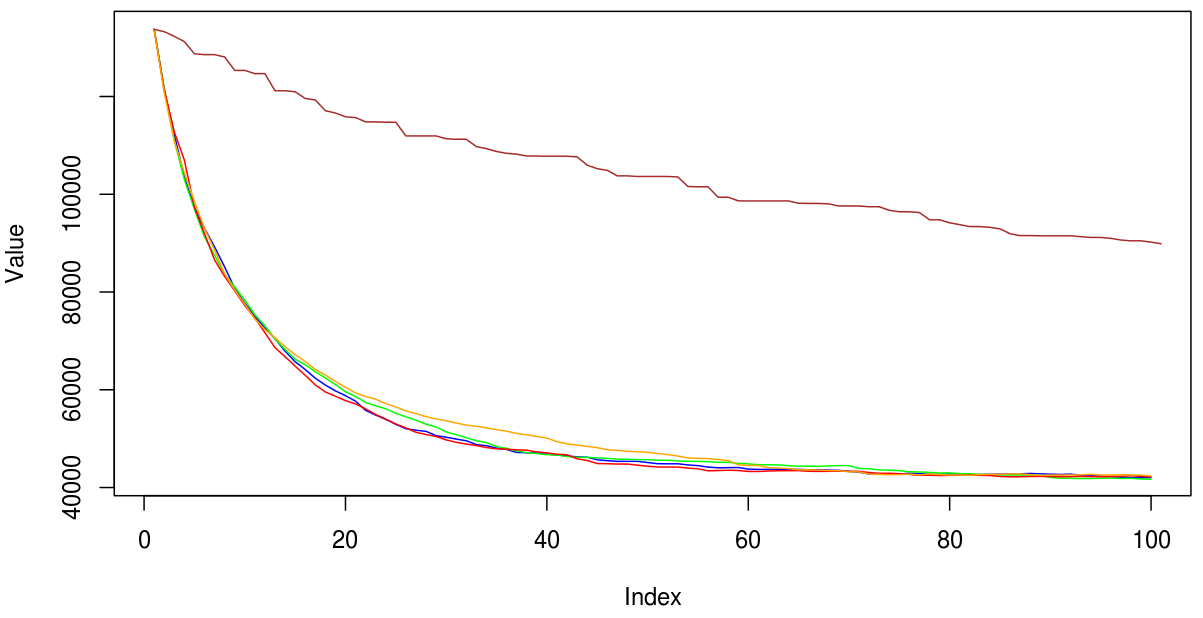
\includegraphics[scale=.35]{tabu_sa.png}
	\caption{Value by step.py}
\end{figure}
\end{center}
In the figure 2, all five algorithms were ran five times to give a mean. The green line is \texttt{tabu3}, the blue one is \texttt{tabu5}, the red one is \texttt{tabu10}, the orange is \texttt{tabu20} and the brown is \texttt{simulated\_annealing}.
\subsubsection{Question 5}
The temperature has an effect on the capability of the value of the found solution to "oscillate". When can thus act on the capability to get out or avoid local optima.
\subsubsection{Question 6}
The higher the length, the less probable it will be for the algorithm to see several times the same solution. It allows also lots of degradation of the value so that getting out of local optima will be easier.
High length or small length both work well as another good path after a local optimum does not require lots of degradation steps.


	
\newpage
	
	
	

\section{Propositional logic}
\subsection{Models and logical connectives}

\subsubsection*{Question 1 : For each sentence, give the number of models that satisfy it (considering the
whole vocabulary).\\}

Since we are using Propositional logic, each variable can be either True or False. Therefore, for each sentences, we have as the number of possibles combinaisons the value 2 power the number of different variables in the sentence. The number of models will be the number of combinaisons which are making the sentence true. \\
This is shown in the following tabulars. \\

\begin {enumerate}
 \item $\beta : (A \vee B) \wedge(B \vee C)$
 \begin{center}

 \begin{tabular}{|c|c|c|c|c||c|}
	\hline
	A & B & C & $A \vee B$ & $B \vee C$& $\beta$ \\
	\hline 
	F & F & F & F & F & F \\
	\hline
	T & T & T & T & T & T \\
	\hline
	F & T & T & T & T & T \\
	\hline
	F & F & T & F & T & F \\
	\hline
	F & T & F & T & T & T \\
	\hline
	T & F & F & T & F & F \\
	\hline
	T & F & T & T & T & T \\
	\hline
	T & T & F & T & T & T \\
 	\hline
 \end{tabular}
 
 \end{center}
 Here we have 5 interpretations which are model of $\beta$
 \item $\beta : A \wedge B$\\
 
 \begin{center}

 \begin{tabular}{|c|c||c|}
	\hline
	A & B & $\beta$ \\
	\hline 
	F & F & F  \\
	\hline
	T & T & T  \\
	\hline
	F & T & F \\
	\hline
	T & F & F \\
	\hline
 \end{tabular}
  
 \end{center}
 
 Here we have 1 interpretation which is model of $\beta$
\item $\beta : (A \Rightarrow B) \Leftrightarrow C $


 \begin{center}

 \begin{tabular}{|c|c|c|c||c|}
	\hline
	A & B & C & $A \rightarrow B$ & $\beta$ \\
	\hline 
	F & F & F & T & F \\
	\hline
	T & T & T & T & T \\
	\hline
	F & T & T & T & T \\
	\hline
	F & F & T & T & T  \\
	\hline
	F & T & F & T & F \\
	\hline
	T & F & F & F & T \\
	\hline
	T & F & T & F & F \\
	\hline
	T & T & F & T & F \\
 	\hline
 \end{tabular}
  
 \end{center}
 Here we have 4 interpretations which are model of $\beta$
\end {enumerate}
\subsubsection*{Question 2 : Give two valid interpretations of the following sentence: $\beta : (A \wedge B) \Rightarrow C$ .}
Two valid interpretation for $\beta$ are :
\begin{center}
\begin{tabular}{|c|c|c|c|}
  \hline
   & \textbf{A} & \textbf{B} & \textbf{C} \\
  \hline
  Interpretation 1 & F & F & F \\
  \hline
  Interpretation 2 & F & F & T \\
  \hline
\end{tabular}
\end{center}
\subsection{Package installation problem}
\subsubsection{Question 1 : Explain how you can express this problem with propositional logic. What are the variables and how do you translate the relations and the query?}
In order to represent the problem, we will declare one variable per package. $I_{i}$, that is set to \texttt{True} if the package $i$ is installed.\\
The three contraints will be expressed as :
\begin{itemize}
  \item Depends : A depends on B : \\
  $$I_{A} \Rightarrow I_{B}$$
  \item Conflicts : Lets be two packages A and B, A conflits with B should be : \\
  $$\neg (I_{A} \wedge I_{B})$$
  \item Provides : It is needed when a package to be installed need a package that is provided by another. As they are possibly several packages that provide the wanted package. A is the wanted virtual package and \{B, C, D\} the packages that provide A : \\
  $$I_{A} \Rightarrow (I_{B} \vee I_{C} \vee I_{D})$$
\end{itemize}

\subsubsection{Question 2 : Translate your model into CNF.}
The point is to have conjunctions of disjunction, we get :
\begin{itemize}
  \item Depends : $\neg I_{A} \vee I_{B}$
  \item Conflicts : $\neg I_{A} \vee \neg I_{B}$
  \item Provides : $\neg I_{A} \vee I_{B} \vee I_{C} \vee I_{D}$
\end{itemize}

\subsubsection{Question 3 : An extension of the problem deals with disjunctive dependencies. For example, package A may depend on B or C, meaning A may be installed if either B or C (or both) is also installed. How can you transform this problem into the basic problem without disjunctive dependencies?}
We can simply write A depends on B or C as : $I_{A} \Rightarrow (I_{B} \vee I_{C})$, which gives as CNF : $\neg I_{A} \vee I_{B} \vee I_{C}$

\subsubsection{Question 7 : To reduce the search space and avoid some unneeded packages in the solution,can you think of lower and upper bounds? Given a list of packages to install, the lower bound are packages that will certainly need to be installed. Every package outside the upper bound is certainly not needed.}
To find a lower bound, when a virtual package is needed, be should make sure that no more than one package providing this virtual package is installed. We can use a \texttt{XOR} statement between the providing package which, for two providers A and B, is written as:
$$(I_{A} \vee I_{B}) \wedge \neg (I_{A} \wedge I_{B})$$
The CNF is : $(I_{A} \vee I_{B}) \wedge (\neg I_{A} \vee \neg I_{B})$\\
To find an upper bound, we can do the opposite by requesting the installation of all providing package for each needed virtual package. We should replace the prodives condition by (for A provided by B and C): 
$$(I_{A} \Rightarrow I_{B}) \wedge (I_{A} \Rightarrow I_{C})$$ 
The CNF is : $(\neg I_{A} \vee I_{B}) \wedge (\neg I_{A} \vee I_{C})$
\end{document}
